\documentclass[12pt,a4paper]{report}
\usepackage[utf8]{inputenc}
\usepackage[brazil]{babel}
\usepackage{graphicx}
\usepackage{hyperref}
\usepackage{abnt-alf}
%\usepackage[alf,abnt-etal-list=0,abnt-etal-cite=3]{abntex2cite}
\usepackage[top=3cm,bottom=2cm,left=3cm,right=2cm]{geometry}
\usepackage{indentfirst}
\usepackage{float}
\usepackage{amsfonts}
\usepackage{url}
\usepackage{tabularx}
\usepackage{color}

\begin{document}
	
	% CAPA
	\pagestyle{empty}
	\begin{center}
		\large  \textbf{UNIVERSIDADE PRESBITERIANA MACKENZIE}
		\large  \textbf{PROGRAMA DE PÓS-GRADUAÇÃO EM}\\
		\large  \textbf{ENGENHARIA ELÉTRICA E COMPUTAÇÃO}\\
		\vskip 8.0cm
		\setlength{\baselineskip}{1.5\baselineskip}
		\textbf{\large CLASSIFICAÇÃO AUTOMÁTICA DO COMPORTAMENTO DINÂMICO DE AUTÔMATOS CELULARES BINÁRIOS}\\
		\vskip 11.0cm
		São Paulo\\
		2018\\
		\vskip 1.0cm
	\end{center}
	
	% CAPA
	\pagestyle{empty}
	\begin{center}
		\large  \textbf{UNIVERSIDADE PRESBITERIANA MACKENZIE}
		\large  \textbf{PROGRAMA DE PÓS-GRADUAÇÃO EM}\\
		\large  \textbf{ENGENHARIA ELÉTRICA E COMPUTAÇÃO}\\
		\vskip 2.0cm
		\textbf{\large Marcelo Arbori Nogueira}\\
		\vskip 4.0cm
		\setlength{\baselineskip}{1.5\baselineskip}
		\textbf{\large CLASSIFICAÇÃO AUTOMÁTICA DO COMPORTAMENTO DINÂMICO DE AUTÔMATOS CELULARES BINÁRIOS}\\
		\vskip 3.0cm
	\end{center}
	\hfill{\vbox{\hsize=8.5cm\noindent\strut
			Projeto de doutorado apresentado ao Programa de Pós-graduação em Engenharia Elétrica e Computação da Universidade Presbiteriana Mackenzie como requisito parcial para obtenção do título de Doutor em Engenharia Elétrica, na área de concentração em Engenharia da Computação.}\\
		\strut}
	\vskip 3.0cm
	\textbf{\normalsize Orientador: Prof. Dr. Pedro Paulo Balbi de Oliveira}\\
	\vskip 2.0cm
	\begin{center}
		São Paulo\\
		2018\\
	\end{center}
	
	\newpage
	\begin{flushright}
		\color{white}.\color{black}
		\vskip 20.0cm
		Aos meus familiares e amigos.

		Dedico.
	\end{flushright}
	
	\newpage
	\pagenumbering{roman}
	\chapter*{Agradecimentos}
	É difícil agradecer a conclusão de uma caminhada tão significante quanto a que busco concluir com este trabalho. Mas é importante destacar o papel de meus pais, que se não puderam me levar pelas mãos, em nenhum momento deixaram de me incentivar. Minhas irmãs, como as melhores amigas, que também me incentivaram e se alegraram com minha decisão de abraçar o desafio de fazer o doutorado.  
	
	O papel de meus colegas do curso também foi muito importante, pois em vários momentos ofereceram seus comentários que muito me auxiliaram, agradeço por isso e espero que nossa amizade permaneça após a conclusão desta caminhada.
	
	Sobretudo agradeço ao meu orientador que sempre esteve presente paciente e dedicado em momentos importantes.

	\newpage
	\pagenumbering{roman}
	\begin{flushright}
		\color{white}.\color{black}
		\vskip 20.0cm
		Histórias de sucesso são raras porque são doloridas.

		(Marcelo Arbori Nogueira)
	\end{flushright}
    	
	% RESUMO
	\newpage
	\thispagestyle{plain}
	\pagenumbering{roman}
	\begin{center}
		\large
		\textbf{RESUMO}
	\end{center}
	\renewcommand{\baselinestretch}{0.6666666}
	Autômatos Celulares apresentam grande variabilidade em suas evoluções temporais não só pela quantidade de regras, mas também pela quantidade de condições iniciais possíveis. Um processo automático para classificar evoluções temporais não só do espaço elementar, como de espaços maiores, é de grande auxílio para as pesquisas na área. 
	
	A classificação automática de imagens, sejam coloridas, em tons de cinzas e até mesmo binárias é bem documentada na literatura e encarar a evolução temporal como uma imagem binária permite utilizar as mesmas técnicas consagradas para a tarefa.
	
	Neste trabalho foram desenvolvidos dois métodos de classificação automática, baseando-se na classificação de Wolfram para o espaço elementar. Ambos os métodos classificam não a regra em si, mas a evolução temporal gerada pela regra.
	
	A primeira abordagem centrou em redes neurais onde a arquitetura convolucional se destacou dentre as demais. O segundo método teve foco no espectro da configurações de vizinhança das células do reticulado. Inicialmente avaliado como extrator de características a serem usadas como entrada da rede feedforward, mostrou-se muito útil ao se desenvolver uma classificação automática com base na distância euclidiana entre espectros.
	\\[0.5cm]
	\begin{flushleft}
		{\bf Palavras-chave:} {\it Autômato celular, rede neural, classificação de comportamento dinâmico, espectro de configuração de vizinhança, rede convolucional, aprendizado profundo.}
		\\[3.0cm]
	\end{flushleft}
	
	% ABSTRACT
	\newpage
	\thispagestyle{plain}
	\pagenumbering{roman}
	\begin{center}
		\large
		\textbf{ABSTRACT}
	\end{center}
	\renewcommand{\baselinestretch}{0.6666666}
	Cellular automata present great variability in their temporal evolutions not only by the amount of rules, but also by the amount of initial conditions possible. An automatic process to classify temporal evolutions not only of the Elementary Space, but of larger spaces, is of great assistance to the researches in the area.
	
	The automatic classification of colored, grayscale and even binary images is well documented in the literature and viewing temporal evolution as a binary image allows us to use the same techniques for the task.
	
	In this work two methods of automatic classification were developed, based on the Wolfram classification for the Elementary Space. Both methods classify not the rule itself, but the time evolution generated by the rule.
	
	The first approach focused on neural networks where the convolutional neural network stood out among the others. The second method focused on the spectrum of the neighborhood configurations of the lattice cells. Initially evaluated as an extractor of characteristics to be used as input feedforward network, it proved very useful when developing an automatic classification based on Euclidean distance between spectra.
	\\[0.5cm]
	\begin{flushleft}
		{\bf Key words:} {\it Cellular automaton, neural network, Fourier transform, classification, neighborhood configuration spectrum.}
	\end{flushleft}
	
	% SUMÁRIO
	\thispagestyle{empty}
	\listof{figure}{Figuras}
	\listof{table}{Tabelas}
	\tableofcontents
	
	% DESENVOLVIMENTO
	\newpage
	\pagestyle{plain}
	\pagenumbering{arabic}
	\renewcommand{\baselinestretch}{1.5}
	\normalsize
	
	
	\chapter{Introdução}
	
	Proposto ainda na década de 1940 como modelo computacional que descrevia a máquina auto-replicante de John von Neumann, os Autômatos Celulares (AC) são também modelos matemáticos com grande capacidade de simulação para incontáveis fenômenos relacionados à física, biologia e ciências sociais. A estrutura de um AC possui um conjunto organizado de células que pode assumir um dos estados de um conjunto finito de estados possíveis. Sendo um sistema dinâmico no tempo, os valores das células mudam segundo uma função que depende da vizinhança da célula. Estes são os elementos comuns de um AC, seja ele unidimensional, bidimensional ou de dimensões maiores \cite{Sarkar:2000:BHC:349194.349202}.
	
	Autômatos celulares são sistemas fortemente emergentes, uma vez que eles possuem propriedades que são irredutíveis e imprevisíveis. Ou seja, não é possível deduzir as propriedades globais a partir das propriedades locais às células, e tão pouco é possível predizer precisamente o estado futuro do sistema a partir de suas partes constituintes. A grande quantidade de unidades, com comportamentos locais, mas que se comunicam e mudam seu estado a depender das informações trocadas, também é uma característica comum de sistemas emergentes como os ACs \cite{Klaus2002}.
	
	Como dito, ele possui grande capacidade de simular uma variedade de fenômenos, mas não são todos que se prestam a qualquer tipo de simulação. Há classes de regras de Autômatos Celulares que se prestam melhor a simulações e outras que simplesmente não são capazes de nada simular, seja por que o estado do reticulado não varia com o tempo ou sua variação está em um estado periódico.
	
	A regra é o que define o comportamento dinâmico do Autômato Celular e para cada uma dela pode-se obter comportamentos dinâmicos dos mais variados. Dentre as regras, delimitar aquelas que são úteis para simulações de fenômenos ou que apresentem comportamento dinâmico interessante a ser pesquisado, como computabilidade, é uma tarefa difícil.
	
	Esta dificuldade se encontra na quantidade de regras que para alguns espaços supera os trilhões, mas também no número de condições iniciais possíveis, que dependendo dos valores, faz com que uma regra apresente comportamento dinâmico distinto do esperado para a sua classe.
	
	Conhecer um espaço de regra em sua totalidade é um problema computacional quase insolúvel dada estas dimensões. Os espaços mais simples podem conter 16, 256 ou até pouco mais de 65500 regra. Acima disso se tem mais de 4 trilhões de regras no espaço considerado. Para se ter uma ideia do que este número significa, suponha que se leve apenas 1s para se avaliar visualmente o comportamento dinâmico de uma regra. Para avaliar todas deste conjunto, se levaria mais de 49000 dias.
	
	Mesmo para um computador nos dias de hoje o processamento é muito pesado. Suponha que a simples chamada de uma função por um programa, sem que a ela faça algo, apenas retorne após ser chamada, leve 3ms. Se esta função for usada para cada uma destas mais de 4 trilhões de regras, levaria em torno de 150 dias para terminar. Pode-se imaginar que qualquer operação incluída nesta função, até uma simples soma, elevaria este tempo consideravelmente.
	
	Esta situação mostra que para conhecer um espaço de regras de um Autômato Celular duas coisas são necessárias. Primeiro, uma abordagem automatizada de avaliação do comportamento dinâmico da regra. Segundo, formas de se reduzir o total de regras que precisam ser avaliadas para se ter uma visão de todo o espaço.
	
	Na sequência do texto, o Capítulo \ref{automatoCelularBinarioUnidimensional} define o que é um AC unidimensional, o Capítulo \ref{cap:classificacaoACBinUni} aborda a classificação de ACs binários encontrada na literatura e os resultados obtidos. No Capítulo \ref{cap:classACUsingNetwork} se aborda a utilização de Redes Neurais Artificiais no aprendizado de características do espaço elementar, com destaque para as Redes Neurais Artificias Convolucionais que possibilitam, como se verá, um aprendizado muito mais preciso das imagens que são a evolução temporal das regras do espaço elementar. No Capítulo \ref{cap:neighborhoodSpectrumAnalises} é proposta uma análise do espaço elementar baseando-se no Espectro de Configuração de Vizinhança e a utilização dos espectros obtidos de cada regra do espaço elementar para a classificação de evoluções temporais binárias. Concluindo, no Capítulo \ref{cap:resultados} é feita uma comparação entre os dois métodos desenvolvidos dando atenção à coerência de ambos os métodos ao serem aplicados no espaço de raio 1.5. Finalmente, no Capítulo \ref{cap:conclusaoCronograma} é feita a conclusão e oferecido um cronograma para os próximos trabalhos.
	
	
	\chapter{Autômato celular binário unidimensional}
	\label{automatoCelularBinarioUnidimensional}
	
	Este trabalho foca em Autômatos Celulares (AC) binários unidimensionais que é constituído pelo reticulado, uma sequência linear de células [$a_0,a_1,a_2,...,a_l$], onde cada célula pode estar em um dos estados do conjunto finito de estados $\Sigma=\{0,1\}$. O valor de cada célula é alterado ao longo do tempo pela ação da função de transição de estado, que a altera segundo o estado da vizinhança analisada. Este estado é o valor da célula central à vizinhança e das células à sua volta, que depende do valor do raio da vizinhança. Pode-se descrever uma transição de estado de uma célula $a_i$ como: $a^{t+1}_i=f(a_{i-r},a_{i-r+1},...,a_i,...,a_{i+r-1},a_{i+r})$. Ou seja, o valor da célula $a_i$ no momento $t+1$ é o resultado da função de transição $f$, onde i é a posição da célula central, $r$ o valor do raio e $t$ o momento discreto que a atualização ocorre \cite{Wolfram1984}.
	
	A função de transição é o que se chama de regra em um AC. Uma regra é um conjunto de transições de estados a partir do estado da vizinhança. Por exemplo $(a_{i-4}=1,a_{i-3}=1,a_{i-2}=0,a_{i-1}=1,a_{i}=0,a_{i+1}=1,a_{i+2}=0,a_{i+3}=0,a_{i+4}=1) = (110101001)\Rightarrow 1$, é uma configuração de vizinhança com 9 células onde o valor da célula central $a_i$ muda para 1 na iteração seguinte; resumidamente; $a^{t+1}_i=f(110101001)=1$. E esta transição ocorre de forma síncrona para todas as células do reticulado, todas são atualizadas no mesmo tempo discreto \cite{2002:NKS:513738}
	
	Uma regra em AC é o conjunto de todas as configurações de vizinhança possíveis com o valor para o qual a célula central transitará na iteração seguinte. Ou seja, uma regra é o conjunto de todas as transições de estado possíveis. Se $r$ for o raio entorno da célula central e $r \in \{0.5, 1.0, 1.5, 2.0, ..., a, a + 0.5, ...\}$, $m = 2r + 1$ é o tamanho da vizinhança. Fazendo $k = |\Sigma|$ o número de estados possíveis que as células do reticulado pode assumir, neste contexto, $k^m$ é o número de configurações de vizinhanças possíveis. E como cada configuração de vizinhança pode transitar para um dos símbolos em $\Sigma$, pode-se calcular a quantidade total de regras possíveis de um AC, calculando todas as configurações de transições possíveis, fazendo $k^{k^m}$ \cite{Martinez_2013}.
	
	O chamado espaço de regras, o conjunto de todas as regras possíveis, no caso dos ACs binários varia apenas conforme o valor do raio $r$, uma vez que a quantidade de estados está fixada em $k = 2$. Se $r = 1$ temos o espaço de regras muito bem estudado por \citeonline{2002:NKS:513738}, denominado espaço elementar. O número de regras deste espaço é $2^{2^3} = 256$. A regra $n$ deste espaço pode variar de 0 a 255. Variando o valor do raio em 0.5, se obtém um espaço de regras com o tamanho $2^{2^4} = 65.536$. Se $r=2$, se tem $2^{2^5} = 4.294.967.296$ regras possíveis. O número de configurações de vizinhança possível cresce exponencialmente com o tamanho da vizinhança $m$, que depende do raio $r$. Já a quantidade de regras possíveis em um espaço cresce exponencialmente com o número de vizinhanças possíveis. Ou, uma pequena variação no valor do raio, se tem uma grande variação na quantidade de regras possíveis.
	
	\citeonline{2002:NKS:513738} organizou as transições de estado como números de base \textit{k}, estando o menor número mais à direita e o maior mais à esquerda. Ao se observar os valores das transições, percebe-se um número, também de base \textit{k}. Este número é utilizado para identificar a regra do AC. A Figura \ref{fig:rule30} mostra o que foi explicado. Os valores binários na primeira linha são as configurações possíveis para a vizinhança em um AC do espaço elementar, enquanto na segunda linha se tem os valores das transições de estado da célula central. Nesta ordem a segunda linha forma o número 30 em binário e este número designa esta regra do espaço elementar.
	
	\begin{figure}[H]
		\centering
		
\includegraphics[scale=1.25]{./img/regra_30_ace}
		\caption{Regra 30 do Autômato Celular Elementar.}
		\label{fig:rule30}
	\end{figure}
	
	Cada regra de um espaço dado apresenta um comportamento dinâmico conforme a regra for executada sobre o reticulado. Este comportamento pode ser visualizado se os estados forem encarados como cores; branco para o valor 0 e preto para o valor 1; e a configuração do reticulado for acumulada e ordenada pelo tempo discreto que a regra é aplicada ao reticulado. O padrão visual que surge, ocorre devido ao comportamento emergente dos ACs, significando que tais padrões globais não se encontram na regra utilizada, que possui programação estritamente local à vizinhança. A Figura \ref{fig:et30} mostra a evolução temporal ao se aplicar a regra definida na Figura \ref{fig:rule30} em um reticulado com 231 células, estados iniciais aleatórios e condição de contorno periódica \cite{2002:NKS:513738}.
	
	\begin{figure}[H]
		\centering
		
\includegraphics[scale=1]{./img/ca_sample_30.png}
		\caption{Evolução temporal da regra 30 em um reticulado com 231 células, condição inicial aleatória, condição de contorno periódica, executado por 693 iterações com 462 passos transientes.}
		\label{fig:et30}
	\end{figure}
	
	Para cada regra utilizada na evolução do AC, emergirá um comportamento dinâmico com características próprias que são úteis no estudo de uma gama ampla de fenômenos, como relatado em \citeonline{RevModPhys.55.601}. Um exemplo de uma característica global de uma regra é a computação universal apresentada pela regra 110 \cite{Neary:2006:PCA:2135489.2135507}. Saber desta propriedade da regra 110 ou de outras características particulares de uma regra, leva à questão sobre a existência de outras regras com a mesma característica.
	
	Sabe-se que o número de regras de um espaço varia muito com uma pequena variação do raio, mas outra fonte de variabilidade é o tamanho do reticulado e como ele é encarado. A regra 60 do espaço elementar é um bom exemplo sobre esta influência. Para qualquer tamanho, a regra apresenta seu comportamento característico, mas para reticulados cujo tamanho seja potência de 2 e a condição de contorno seja periódica, resulta após um período transiente, em uma evolução temporal homogênea. E esta característica é compartilhada com as regras 90, 102, 153, 165 e 195. A evolução temporal de cada uma pode ser visto na Figura \ref{fig:rulesHomoPow2}.
	
	\begin{figure}[H]
		\centering
		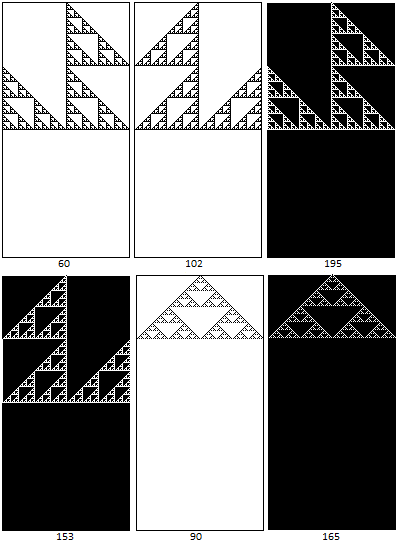
\includegraphics[scale=1]{./img/rules_homogeneous_pow2.png}
		\caption{Regras caóticas do espaço elementar com evolução temporal homogênea após período transiente com o mesmo tamanho do reticulado ou com a metade dele.}
		\label{fig:rulesHomoPow2}
	\end{figure}
	
	Outra fonte de variabilidade no comportamento das regras guarda relação com o estado inicial do reticulado, mesmo sem um tamanho específico definido. A regra exibida na Figura \ref{fig:rule30} possui comportamento caótico; no entanto, se o estado inicial do reticulado for todas as células com valor 0 (cor branca), a evolução temporal resultante se equivale a uma regra homogênea que leve todas as células a 0.
	
	A regra 62 do espaço elementar é outro exemplo de mudança aparente do comportamento da regra devido a configurações iniciais distintas. A Figura \ref{fig:rule62WithiTwoInitialConditions} exibe duas evoluções temporais obtidas pela regra 62 com características distintas. Enquanto à esquerda se percebe uma evolução temporal com características periódicas, à direita se observa uma evolução temporal com características complexas, apresentando estrutura que remete a características caóticas \cite{Weifeng2014}.
	
	\begin{figure}[H]
		\centering
		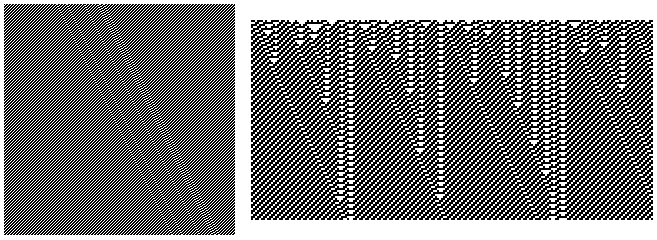
\includegraphics[scale=1]{./img/ca_sample_62.png}
		\caption{Duas evoluções temporais para a regra 62 com resultados distintos. À esquerda uma evolução temporal periódica e à direita uma evolução temporal com características complexas.}
		\label{fig:rule62WithiTwoInitialConditions}
	\end{figure}
	
	O tamanho do reticulado também contribui para a variabilidade do sistema, pois dado um reticulado de tamanho $l$ as condições iniciais possíveis são $k^l$. Isso quer dizer que o número de condições iniciais possíveis aumenta exponencialmente com o tamanho do reticulado. Para um reticulado com, por exemplo, 100 células, o número de condições iniciais é tão grande que existe uma chance de encontrar condições iniciais que ao aplicar uma determinada regra sobre ele, a evolução temporal não apresente o comportamento típico da regra.
	
	Apesar dos ruídos inerentes ao processo, classificar o conjunto de regras de um espaço é um bom meio para se agrupar regras com características semelhantes. Existem vários algoritmos voltados para o agrupamento que poderiam ser usados para se agrupar automaticamente as regras e assim se investigar as propriedades comuns de cada grupo. Porém, no caso dos ACs estas propriedades não podem ser completamente classificadas \cite{Culik:1988:UCC:45269.45271}. Contudo, isso não impede a elaboração de uma classificação tão precisa quanto possível.
	
	O espaço elementar é um espaço muito estudado e conhecido. Por ser relativamente pequeno, uma classificação deste espaço pode ser obtida, mesmo de forma manual, analisando a evolução temporal de cada regra. \citeonline{Wolfram1984} propôs uma classificação para o espaço elementar com 4 classes, coda uma das quais, enumeradas a seguir.
	
	\begin{enumerate}
		\item A evolução leva a um estado homogêneo;
		\item A evolução leva a um conjunto de estruturas simples e estáveis ou periódicas;
		\item Evolução leva a um padrão caótico;
		\item A evolução leva a estruturas localizadas complexas, às vezes de longa duração.
	\end{enumerate}
	
	Representando a regra como na Figura \ref{fig:rule30}, é possível realizar três operações sobre as transições das 8 vizinhanças possíveis, como conjugação; a troca dos valor de 1 para 0 e de 0 para 1. Reflexão; inverter os valores das transições, onde o primeira se torna a última, a penúltima a segunda e assim por diante. Reflexão e Conjugação; que é a troca de seus valores e inversão da ordem. A regra $10010100_2 = 148_{10}$ pode ter os valores das transições invertidos e se obter a regra $01101011_2 = 107_{10}$ e aplicando as duas operações se obtém a regra $11010110_2 = 214_{10}$.
	
	Repetindo as mesmas operações para as 256 regras possíveis do espaço elementar, se obtém para cada regra um conjunto de regras equivalentes a ela. Ao retirar destes grupos as regras com menor valor, tem-se 88 classes de regras com comportamento dinâmico equivalentes, como organizado na Tabela \ref{table:dynamicEquivalentRules}.
	
	\begin{table}[H]
		\caption{Regras dinamicamente equivalentes do espaço elementar.}
		\label{table:dynamicEquivalentRules}
		\begin{tabularx}{\textwidth}{|l|X|}
			\hline
			Classe I & 0, 8, 32, 40, 128, 136, 160, 168 \\
			Classe II & 1, 2, 3, 4, 5, 6, 7, 9, 10, 11, 12, 13, 14, 15, 19, 23, 24, 25, 26, 27, 28, 29, 33, 34, 35, 36, 37, 38, 42, 43, 44, 46, 50, 51, 56, 57, 58, 62, 72, 73, 74, 76, 77, 78, 94, 104, 108, 130, 132, 134, 138, 140, 142, 152, 154, 156, 162, 164, 170, 172, 178, 184, 200, 204, 232 \\
			Classe III & 18, 22, 30, 45, 60, 90, 105, 122, 126, 146, 150 \\
			Classe IV & 41, 54, 106, 110 \\
			\hline
		\end{tabularx}
	\end{table}
	
	Classificar as 88 representantes das classes de equivalência é o suficiente para classificar todo o espaço, uma vez que ao classificar um das 88, a classificação das demais regras do classe está definida. O mesmo é verdade para espaços maiores que o elementar, ao classificar o subconjunto de regras dinamicamente equivalentes, todo o espaço estará classificado \cite{Wolfram1986}.
	
	Naturalmente a classificação de Wolfram não é única, e outras podem ser propostas, como a classificação de \citeonline{Li90thestructure}. Ambas não descrevem completamente o espaço elementar, mas são tão precisas quanto possível, para os propósitos a que se prestam. Mas como o espaço de regras tem crescimento duplamente exponencial dependente do raio, expandir qualquer classificação aplicada ao espaço elementar para outros maiores é tarefa manualmente impraticável.
	
	Qualquer classificação não se presta a ser aplicada apenas ao espaço elementar, pois conhecer espaços maiores permitiria encontrar características que não se encontram no espaço elementar. Mas, como mencionado, uma classificação manual de espaços maiores não é viável. Aplicar sobre espaços maiores algoritmos de classificação também não é o desejado por construir uma classificação que não necessariamente guarda relação com alguma classificação conhecida e assim impossibilitar comparações entre espaços distintos.
	
	A evolução temporal de qualquer autômato celular binário, independente de seu raio, pode ser representada por uma matriz binária, sendo esta a estrutura usada para representar as evoluções temporais neste trabalho. Não havendo distinção estrutural entre evoluções temporais geradas por espaços distintos, os meios de se classificar automaticamente as regras do espaço elementar segundo a classificação de \citeonline{Wolfram1984}, usada aqui como referência, pode ser aplicada indistintamente a qualquer evolução temporal.
	
	Avalia-se aqui a possibilidade de, ao se desenvolver meios de classificação automática baseados nas evoluções temporais geradas pelas regras do espaço elementar, de form que a classificação automática possa ser levada para espaços maiores, mantendo uma acurácia elevada, sem que se tenha maiores informações sobre este espaço que não seja o tamanho de seu raio.
	
	Isso quer dizer que processo desenvolvido será uma ferramenta para gerar informações sobre um espaço desconhecido. Por isso deve ser capaz de se adaptar para os casos não observados, pois é possível que espaços maiores tenham comportamentos não existentes no espaço elementar. Desta forma, será possível conhecer melhor espaços que hoje são parcialmente ou totalmente desconhecidos, tendo como informação apenas a evolução temporal gerada por suas regras. O próximo capítulo aborda a classificação de ACs Binários Unidimensionais.
	
	
	\chapter{Classificação de autômatos celulares binários unidimensionais}
	\label{cap:classificacaoACBinUni}
	
	A definição de uma imagem pode ser feita usando uma função de duas dimensões, $I = f(x, y)$, onde as coordenadas x e y correspondem à posição do pixel e o valor da função à cor presente no ponto. O processamento deste conjunto de informações, ou processamento de imagens possui aplicação diversas em várias áreas como medicina; astronomia; automação em vários aspectos; sistema de inspeção visual automática; interpretação de cena remotamente detectada; técnicas de imagem biomédica; vigilância de defesa; recuperação de imagem baseada em conteúdo; acompanhamento de objetos em movimento; compressão de imagem e vídeo. Uma das tarefas realizadas é o reconhecimento da imagem, que permite associar a imagem a um identificador, permitindo alguma tomada de decisão a partir desta associação \cite{Acharya:2005:IPP:1088917}.
	
	\citeonline{Gonzales:1987:DIP:22881} definem alguns passos fundamentais no processamento de imagens, se iniciando com a aquisição da imagem; melhorar a qualidade da imagem, processamento das cores; compressão; processos ligados a morfologia e segmentação; representação e descrição da imagem; e reconhecimento. Este último de grande interesse para este trabalho.
	
	O processo de captura de imagem contém muitos ruídos provenientes de várias fontes. Desde a iluminação inadequada até borrões causados pelo movimento, passando por interferências externas como a que a atmosfera causa nas imagens astronômicas. Para melhorar a qualidade das imagens pode-se usar métodos no domínio espacial ou da frequência, onde o domínio espacial se refere ao plano da imagem enquanto a frequência tem relação com mudanças sob a representação da imagem em suas frequências, obtida pela transformada de Fourier, por exemplo \cite{Gonzales:1987:DIP:22881}.
	
	No domínio espacial pode-se aplicar sobre a imagem uma transformação do nível de cinza: que é a transformação do valor de cada pixel fazendo $s = T(r)$, onde \textit{r} é o valor inicial e o final; processamento de histograma: que calcula a proporção de cada intensidade possível para os pixeis, obtendo-se a probabilidade de cada intensidade ocorrer na imagem; operações aritméticas ou lógicas: que aplica operações lógicas sobre uma imagem ou operações aritméticas entre duas imagens, como a subtração das duas; e filtros espaciais: que implica em operações de vizinhança utilizando uma sub-imagem de mesmo tamanho da vizinhança. Estes processos podem ser combinados a depender dos objetivos desejados na melhoria da qualidade da imagem, que é uma tarefa muito direcionada ao problema.
	
	A melhora da imagem usando o domínio da frequência envolve o uso de transformadas do domínio espacial. Aqui se aborda as possibilidade do uso da transformada de Fourier, que descreve a imagem em suas frequências, onde a intensidade para cada frequência é o coeficiente do seno ou cosseno que forma a imagem no domínio espacial e de posse da imagem transformada pode-se aplicar filtros de frequência. Um filtro passa-alta, que filtra as frequências abaixo de um limiar e permite que as acima dele permaneçam. Isto permite destacar as bordas ao restaurar a imagem a partir das frequências filtradas, pois as altas frequências são causadas pela transição entre uma área da imagem para outra, criando uma borda. Já um filtro passa-baixa destacaria as regiões homogêneas da imagem.  
	
	É possível relacionar a evolução temporal a uma imagem, porém comparada com uma imagem capturada por uma câmera por exemplo, a imagem da evolução temporal é extremamente mais simples com relação a ruídos provenientes da captura, pois tal imagem não é capturada, mas sim gerada por um processo computacional. Isso aproxima a obtenção desta imagem à computação gráfica, já que a imagem foi gerada a partir de informações fornecidas a um algoritmo.
	
	Outra simplificação da imagem da evolução temporal de ACs binários é quanto à inexistência de cores, ou mesmo tons de cinza, já que apenas pixel pretos ou branco, são possíveis, representando os números 1 e 0, respectivamente. Assim, a tarefa de se classificar uma evolução temporal se reduz a classificar uma imagem preto-e-branco se a própria evolução for encarada como uma imagem binária. Tal imagem pode ser mais simples se levarmos em consideração o número de canais e cores, no caso existe apenas um canal e não 3 como em uma imagem colorida.
	
	Aqui aborda-se dois métodos para a classificação de imagens, a extração de características da imagem que possibilite a construção de um vetor de característica a ser utilizado em um processo de decisão, ou a utilização de redes neurais que podem ter a própria imagem como entrada ou usar o vetor de características para o treinamento.
	
	Em \citeonline{JassemAndHamid2012} foi utilizado um vetor de características como entrada tanto em uma árvore de decisão quanto a rede neural desenvolvida para a tarefa de classificação. A Figura \ref{fig:RedeNeuralRBFDocClass} mostra a rede neural utilizada, com parte de suas ligações, uma vez que a rede é completamente conectada. \citeonline{JassemAndHamid2012} relata que o uso desta abordagem permitiu acurácia de 96\% na classificação de documentos como fotos, textos e composto.
	
	\begin{figure}[H]
		\centering
		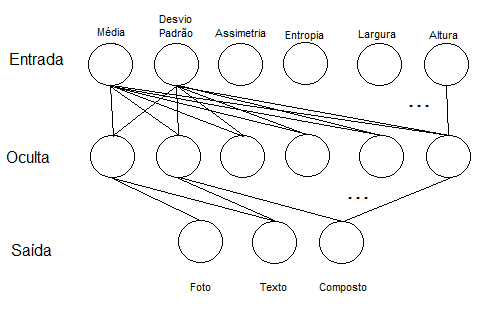
\includegraphics[scale=1]{./img/rede_neural_RBF_doc_class.png}
		\caption{Rede neural RBF utilizada na classificação de documentos digitais.}
		\label{fig:RedeNeuralRBFDocClass}
	\end{figure}
	
	O vetor de característica $\vec{v}_i=(\mu_i,\sigma_i,s_i,H_i,Y_i,X_i)$ se refere às características de um dos canais de cores da imagem. Ele é composta pela intensidade média do canal, Equação \ref{eq:mediaCorImag}, onde i é o canal e $P_{ij}$ é a probabilidade de ocorrência de um pixel com intensidade j; pelo desvio padrão da intensidade de cores, Equação \ref{eq:desvpadCorImag}; o valor de assimetria média do canal, Equação \ref{eq:skewnessCorImag}; e entropia do canal, Equação \ref{eq:entropyCorImag}; e as dimensões da imagem, altura $Y_i$ e largura $X_i$. Este mesmo vetor serviu para a tomada de decisão através de uma árvore de decisão, e também como entrada da rede neural. No caso de uma evolução temporal, há apenas um canal, logo as medidas dizem respeito a toda a imagem.
	
	\begin{equation}
	\mu_i = \frac{1}{N}\times \sum_{j=1}^{N}P_{ij}
	\label{eq:mediaCorImag}
	\end{equation}
	
	\begin{equation}
	\sigma_i=\sqrt{\left ( \frac{1}{N}\sum_{j=1}^{N}\left ( P_{ij}-\mu_i \right )^2 \right )}
	\label{eq:desvpadCorImag}
	\end{equation}
	
	\begin{equation}
	s_i=\sqrt[3]{\left ( \frac{1}{N}\sum_{j=1}^{N}\left ( P_{ij}-\mu_i \right )^3 \right )}
	\label{eq:skewnessCorImag}
	\end{equation}
	
	\begin{equation}
	H_i=-\sum_{j=1}^{N}P_{ij}log_2 P_{ij}
	\label{eq:entropyCorImag}
	\end{equation}
	
	Em \citeonline{JassemAndHamid2012} a entropia foi calculada para todo o canal, servindo como um dos parâmetros do vetor de características. Mas também é possível utilizar a variação da entropia ao longo da evolução temporal e utilizar sua variação para classificar a evolução temporal de acordo com a variação obtida. Ou seja, a cada passo o reticulado está em um estado, que muda ao longo do tempo. Medindo a entropia do reticulado para cada momento discreto se obtém a variação de sua entropia ao logo do tempo. A classificação é possível relacionando a média da entropia para uma regra com o desvio-padrão obtido, obtendo-se regiões onde cada classe de regra é mais frequente \cite{Andrew1998}. 
	
	
	\chapter{Classificação de autômatos celulares utilizando redes neurais artificiais}
	\label{cap:classACUsingNetwork}
	
	Redes neurais parecem ser a solução natural, desenvolvida ao longo de bilhões de anos de evolução biológica, para o processamento de informações, estando mesmo presente nas formas mais simples de vida do planeta. O sistema nervoso central recebe estímulos variados do ambiente, processa esta informação e reage, possibilitando não só uma reação física do indivíduo, mas também adaptações hormonais regulatórias do funcionamento do corpo.
	
	Tanto nos seres humanos quanto em outros animais a visão é um sentido fundamental e sendo a visão uma tarefa de processamento de informações, utilizar redes neurais artificiais para desenvolver soluções neste campo é esperado. Por este motivo, uma das áreas onde redes neurais são muito utilizadas é o processamento de imagem para auxílio das mais variadas tarefas. Há aplicações, por exemplo em auxílio a diagnóstico médico através de exames por imagens, e  auxílio a monitoramento remoto por satélite, vigilância de estradas e identificação de veículos conduzido por infratores. Em todas estas aplicações a tarefa de classificar as imagens analisadas está presente, mostrando a grande capacidade para solucionar este tipo de problema via redes neurais artificiais.
	
	A evolução temporal de um AC binário é uma matriz que contém zeros e uns. Esta matriz pode ser tratada como uma imagem binária, conforme exposto na Figura \ref{fig:et30}, onde o valor 0 é tratado como branco e 1 com preto e, desta forma, exibindo o padrão da figura. Sobre ela pode-se usar técnicas de classificação de imagens auxiliada por rede neural artificial.
	
	A capacidade de mapear a entrada para uma saída via treinamento, a adaptatividade da rede a situações não treinadas, e a tolerância a falha, proveem robustez ao funcionamento da rede. Estas características são úteis na classificação de ACs binários devido à variabilidade associada às evoluções temporais, mesmo que geradas por uma mesma regra, pois a evolução temporal muda se as condições iniciais mudarem. E também, como o número de condições iniciais possíveis é comumente grande, é possível classificar corretamente uma evolução temporal não apresentada à rede. Ou seja, mesmo para um espaço de evoluções temporais possíveis extremamente grande, a rede neural tende a oferecer uma resposta dentro de uma faixa de acerto desejada.
	
	Nas seções seguintes define-se com mais detalhes o que é e quais são os componentes de uma rede neural, além de se explorar a arquitetura das redes neurais utilizadas para abordar o problema de classificação dos Autômatos Celulares binários.
	
	
	\section{Componentes de Uma Rede Neural Artificial}
	
	Uma rede neural é uma tripla $R=\{N,V,w\}$, onde $N$ é o conjunto de neurônios da rede; $V$ é o conjunto de vértices que ligam dois neurônios; e $w: V \Rightarrow \mathbb{R}$ é uma função que recebe os índices de dois neurônios e retorna a intensidade da conexão, esta valendo $w_{i,j}$. Sendo $i$ índice do neurônio origem e $j$ o neurônio destino da conexão.
	
	Um neurônio possui um conjunto de estímulos que podem ser a saída de outros neurônios ou ser um estímulo externo à rede, e neste caso o neurônio que recebe este estímulo é denominado neurônio de entrada. Estes estímulos de entrada do neurônio são a entrada da função de propagação. Esta é a entrada para a função de ativação, que é a entrada para a função de saída do neurônio. A Figura \ref{fig:NeuronioArtificial} resume em um diagrama a estrutura de um neurônio artificial. Nela se vê a função de propagação $\sigma$, a função de ativação $a(.)$ e a função de saída $out(.)$. A função linear é comumente usada como função de saída onde $y_j=a(net_j)$ \cite{haykin2009neural}. 
	
	\begin{figure}[H]
		\centering
		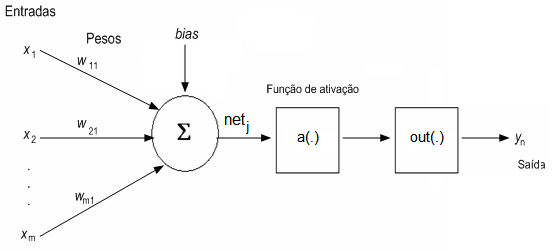
\includegraphics[scale=1]{./img/neuronio_artificial.png}
		\caption{Diagrama de um neurônio artificial destacando suas três partes constituintes principais. As funções de propagação, ativação e saída.}
		\label{fig:NeuronioArtificial}
	\end{figure}
	
	Já o conjunto $X$ de valores $x_i$, diz respeito aos estímulos de entrada do neurônio, e o conjunto $W$ de valores $w_{ij}$, a intensidade de ligação do neurônio com cada entrada ou outros neurônio; a entrada da rede que o neurônio $j$ recebe ($net_j$) é calculada pela função de propagação da Equação \ref{eq:propagation_function}.
	
	\centerline{$net_{j}=f(x_1,x_2,...,x_n,w_1,w_2,...,w_n)$}
	\begin{equation}
	net_{j}=f(X,W)
	\label{eq:propagation_function}
	\end{equation}
	
	É comum usar uma soma dos valores de entrada, ponderada pelos pesos e adicionando o valor do bias, como a função de propagação definida globalmente para a rede. Ou seja, todos os neurônios da rede possuem a mesma função de propagação conforme a Equação \ref{eq:weighted_sum}.
	
	\begin{equation}
	net_{j}=\sum_{i \in I}\left ( x_i \cdot w_{ij} + b_j \right )
	\label{eq:weighted_sum}
	\end{equation}
	
	Mas se o valor do bias for encarado como um dos valores de entrada fazendo $b_j=1$, $x_0=b_j$ e $w_{0j}=b_j$, a Equação \ref{eq:weighted_sum} pode ser reescrita como a Equação \ref{eq:weighted_sum_without_bias}.
	
	\begin{equation}
	net_{j}=\sum_{i \in I}\left ( x_i \cdot w_{ij} \right )
	\label{eq:weighted_sum_without_bias}
	\end{equation}
	
	A função de propagação transforma os vetores de entrada e peso em um escalar. Este escalar é a entrada da função de ativação, que emula a ativação que ocorre no neurônio natural ao receber estímulos. Devido ao fato de a função de saída do neurônio ser uma função linear, na prática a função de propagação acaba sendo a função de saída.
	
	Há várias opções para a função de ativação que simule a ativação do neurônio após um limiar. Pode-se utilizar a função degrau (\ref{eq:funcao_degrau}), a função logística (\ref{eq:funcao_tg_hiperbolica}) que é um caso particular da função de Fermi (\ref{eq:funcao_fermi}). A Figura \ref{fig:FuncoesAtivacoes} mostra os respectivos gráfico de cada função.
	
	\begin{equation}
	a(net_j)=\left \{ 
	\begin{array}{l c l}
	0 & se & net_j \leq 0 \\ 
	1 & se & net_j > 0
	\end{array}
	\right.
	\label{eq:funcao_degrau}
	\end{equation}
	
	\begin{equation}
	a(net_j)=tanh(net_j)=\frac{e^{net_j}-e^{-net_j}}{e^{net_j}+e^{-net_j}}
	\label{eq:funcao_tg_hiperbolica}
	\end{equation}
	
	\begin{equation}
	a(net_j)=\frac{1}{1+e^{\frac{-net_j}{T}}}
	\label{eq:funcao_fermi}
	\end{equation}
	
	\begin{figure}[H]
		\centering
		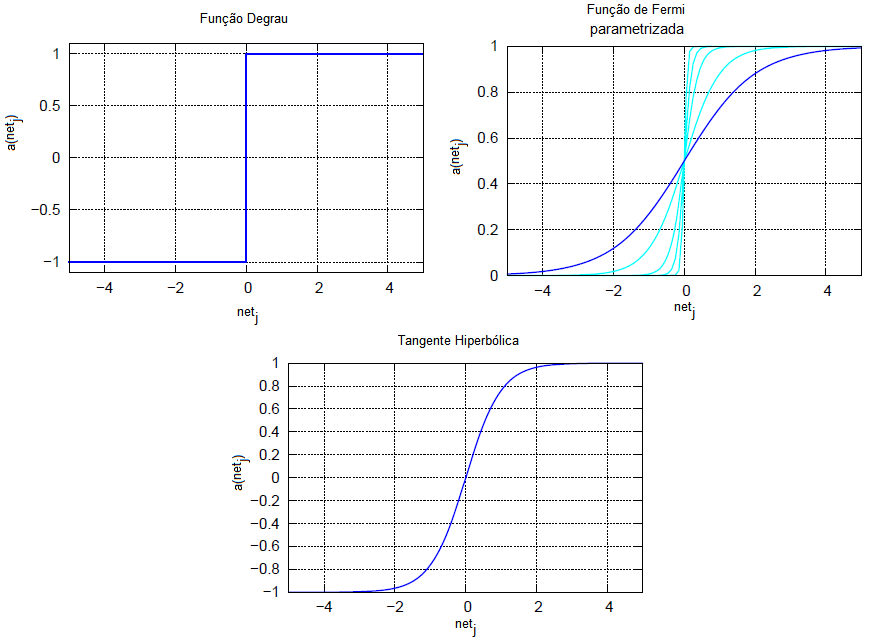
\includegraphics[scale=0.53]{./img/funcoes_ativacoes.png}
		\caption{Funções comumente utilizadas como função de ativação de um neurônio artificial.}
		\label{fig:FuncoesAtivacoes}
	\end{figure}
	
	Pela Figura \ref{fig:FuncoesAtivacoes} pode-se observar que cada uma das funções de ativação possui um limiar, acima do qual o neurônio está ativo, e abaixo, o neurônio está inativo. Esta saía estimulará os neurônios seguintes, cada um dos quais possuindo a mesma estrutura apresentada aqui. 
	
	Um neurônio artificial ou perceptron, conforme o exposto, possui capacidade para classificar um conjunto de dados em duas classes distintas. Caso se use mais de um neurônio, é possível a classificação de mais de uma classe. No entanto, o problema de classificação precisa ser linearmente separável. O problema de classificação é resolvido ajustando os pesos sinápticos dos neurônios até que a resposta observada esteja dentro do esperado.
	
	No entanto, para a tarefa de classificação que se pretende neste trabalho, um separador linear não é suficiente uma vez que há comportamentos não-lineares para os Autômatos Celulares. Assim é necessária a utilização de mais de uma camada de neurônios para solucionar adequadamente o problema, que é a classificação da evolução temporal nas 4 classes definidas por \citeonline{Wolfram1984}
	
	Uma rede feedforward é uma rede com vários neurônios organizados em camadas, onde a primeira camada recebe o estímulo inicial e gera uma saída, a qual serve de entrada para a camada seguinte, e o processo continua até a camada de saída, que gera o resultado do processamento da rede. Neste tipo de rede os neurônios de uma camada são totalmente ligados com os neurônios da camada seguinte. A Figura \ref{fig:RedeNeuralMulticamadas}
	
	\begin{figure}[H]
		\centering
		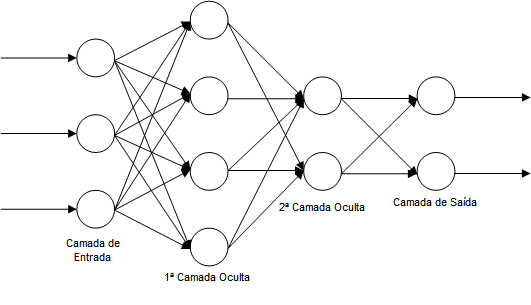
\includegraphics[scale=0.70]{./img/rede_neural_multicamadas.png}
		\caption{Rede feedforward com duas camadas oculta, 3 neurônios na entrada e 2 na saída.}
		\label{fig:RedeNeuralMulticamadas}
	\end{figure}
	
	Mas para este tipo de rede, no contexto de uma tarefa de classificação, faz-se necessário a extração de características relacionadas a cores, formas e textura, por exemplo. Já para uma rede artificial convolucional não há a necessidade de se extrair características das imagens, podendo submeter à rede exatamente a imagem a ser classificada.
	
	A próxima seção apresenta os resultados de classificação de evoluções temporais utilizando uma rede feedforward tendo como entrada a potência do espectro de Fourier. Na sessão seguinte será relatada a utilização de uma rede neural convolucional na tarefa de classificação.
	
	
	\section{Rede Neural Artificial Feedforward, Transformada de Fourier e Classificação}
	
	\citeonline{Kunkle2003} usou uma rede feedforward e um vetor de características para classificar ACs segundo a classificação em \citeonline{Li90thestructure}, obtendo resultado superior a 98\% de acurácia. Aqui, o vetor de características será obtido através da transformada de Fourrier, com o intuito de se ter um processo não subjetivo de escolhas dos componentes do vetor de características. 
	
	A transformada de Fourrier é uma ferramenta muito utilizada para o tratamento de imagens. Ela permite a construção de filtros que permitem isolar ou destacar elementos da imagem ou eliminar ruídos. Quando a imagem é reconstruída a partir do espectro de frequência gerado pela transformada, a imagem reconstituída pode destacar apenas os elementos de interesse ou possuir menos ruído.
	
	Nesta seção descrevem-se os resultados obtidos ao se utilizar a transformada de Fourier como um extrator de características da evolução temporal. A transformada pode ser usada para transformar a evolução temporal dada em uma representação no domínio da frequência e submeter a parte mais relevante a uma rede feedforward para a classificação \cite{Gonzales:1987:DIP:22881}. 
	
	A evolução temporal como uma imagem binária submetida à Transformada Discreta de Fourier de duas dimensões, explicitada na Equação \ref{eq:TransformadaFourrier}, resulta em uma representação no domínio da frequência, que pode ser revertida utilizando a transformada inversa da Equação \ref{eq:TransformadaInversaFourrier}.
	
	\begin{equation}
	F(u,v)=\frac{1}{MN}\sum_{x=0}^{M-1}\sum_{y=0}^{N-1}f(x,y)e^{-j2\pi}(\frac{ux}{M}+\frac{vy}{N})
	\label{eq:TransformadaFourrier}
	\end{equation}
	
	\begin{equation}
	f(x,y)=\sum_{u=0}^{M-1}\sum_{v=0}^{N-1}F(u,v)e^{j2\pi}(\frac{ux}{M}+\frac{vy}{N})
	\label{eq:TransformadaInversaFourrier}
	\end{equation}
	
	A ideia central da transformada é a possibilidade de se representar qualquer sinal como uma soma de senos e cossenos. A transformada então resulta em uma matriz complexa onde cada elemento representa uma frequência e seu valor guarda relação com a amplitude do seno ou cosseno naquela frequência. Uma forma de se analisar visualmente os valores em cada frequência é calcular a potência do  espectro de Fourier, dada na Equação \ref{eq:PotenciaEspectroFourrier}.
	
	\begin{equation}
	|X(u,v)| = \sqrt{real(u,v)^2 + img(u,v)^2}
	\label{eq:PotenciaEspectroFourrier}
	\end{equation}
	
	Ao ser aplicada sobre a imagem, que está no domínio do tempo, obtém-se uma matriz com as informações da imagem no domínio da frequência. As frequências mais baixas contém informações referentes aos detalhes da imagem, enquanto as frequências mais altas contém informações referentes aos contornos, pois são mudança abruptas nas imagens. O procedimento de filtragem que elimina as frequências mais altas e mantém as mais baixas utiliza um filtro denominado passa-baixa, justamente por deixar passar apenas as frequências mais baixas e eliminar as mais altas. Já um filtro passa-alta deixa apenas as altas frequências passarem enquanto bloqueia as mais baixas. Por fim, um filtro passa-faixa aceita apenas frequência dentro de uma faixa pré-determinada e bloqueia as outras \cite{Haykin:1998:SS:552094}.
	
	A denominação do filtro depende dos limiares escolhidos e as frequências aceitas que podem estar acima ou abaixo dos limiares definidos, ou entre eles. Falar de contornos em uma evolução temporal não necessariamente faz sentido e para a tarefa de classificação se poderia escolher as baixas frequências da imagem, uma vez que as altas frequências ocorrem devido aos contornos.  
	
	A \ref{fig:RuleAndSpectro_109_110} mostra duas evoluções temporais, das regras 109 e 110 respectivamente e abaixo de cada uma a imagem formada pelo espectro de potência da transformada de Fourier  referente às evoluções temporais das referidas regras. 
	
	\begin{figure}[H]
		\centering
		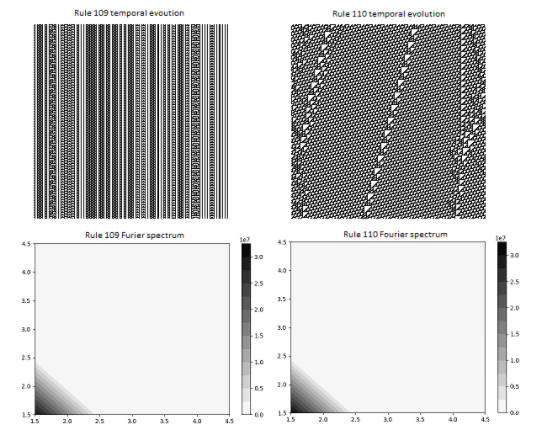
\includegraphics[scale=1.0]{./img/rule_and_spectro_109_110.png}
		\caption{Evoluções temporais das regras 109 e 110, respectivamente classes 2 e 4 da classificação Wolfram. Abaixo de cada uma seus respectivos espectros de Fourier limitados para frequências inferiores a 5, tanto no eixo vertical quanto no horizontal da imagem.}
		\label{fig:RuleAndSpectro_109_110}
	\end{figure}
	
	Ao analisar os espectros de Fourier para as transformadas das evoluções temporais das regras do espaço elementar, ficou claro que frequências superiores a 5 em ambos os eixos da imagem não continham muita informação e por isso se optou por um filtro passa-baixa e se adotou 5 como limiar deste filtro.
	
	Ao se fazer uma análise de um sinal no domínio da frequência normalmente se filtra o sinal para então reconstruí-lo, suavizado ou com destaques para os contornos da imagem, por exemplo. Porém a abordagem usada aqui não reconstitui a evolução temporal, já que o próprio espectro de potência da transformada de Fourier foi utilizado como entrada da rede, que apesar da pouca distinção visual exibida na Figura \ref{fig:RuleAndSpectro_109_110}, foi suficiente para o treinamento da rede feedforward. A Figura \ref{fig:EvolucaoErroFeedforward} mostra a evolução típica do erro da rede durante o treinamento.
	
	\begin{figure}[H]
		\centering
		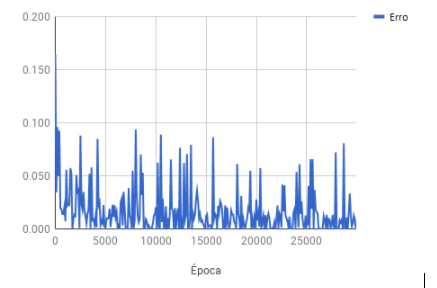
\includegraphics[scale=1.0]{./img/evolucao_erro_feedforward.png}
		\caption{Evolução típica do erro durante o treinamento da rede feedforward utilizando o espectro de potência da transformada de Fourier como entrada.}
		\label{fig:EvolucaoErroFeedforward}
	\end{figure}
	
	O valor do erro mostrou grande variabilidade durante os treinos, porém a acurácia da rede apresentou valores entre 93\% e 96\%, com erro nos treinos chegando a 3.310-7 para 30.000 ciclos de treinamento. Para 10.000 ciclos de treinamento chegou-se a 79.7\% de acurácia com erro ao fim do treinamento chegando a 3.310-6. Para 50.000 ciclos de treinamento a acurácia foi de 74.4\%, com erro durante o treino chegando a 2.910-14. Os resultados obtidos indicam que por volta de 30.000 ciclos de treinamento obtém-se a melhor acurácia da rede.
	
	O uso da transformada de Fourier mostrou ser capaz de apresentar bons resultados na classificação de evoluções temporais das regras do espaço elementar. No entanto, a possibilidade de generalização do processo de classificação e classificar evoluções temporais geradas por regras de espaços maiores, ainda está inconclusivo, sendo necessários mais testes com a rede treinada, ou até mesmo revisão do processo de treinamento ou do formato dos dados utilizados no processo.
	
	Na próxima seção serão descritos os resultado obtidos ao utilizar redes neurais convolucional. Neste tipo de rede, quando utilizada para classificar imagens, a própria imagem pode ser utilizada como entrada da rede, sem a necessidade de se obter vetores de características.
	
	
	\section{Rede Neural Artificial Convolucional e Classificação de Evoluções Temporais}
	
	Redes neurais convolucionais (CNN - Convolutional Neural Network) são redes neurais multi-camadas com estrutura distinta das redes feedforward, utilizadas na classificação de ACs binários à seção anterior. O primeiro ponto importante é o fato de que em uma CNN a entrada é bidimensional, enquanto na rede feedforward o espectro de potência da transformada de Fourier foi linearizado para formar o vetor de entrada \cite{Goodfellow-et-al-2016}.
	
	Em uma CNN não há a necessidade de se extrair características da imagem e gerar um vetor (no caso das CNNs, um plano) de entrada, pois a própria estrutura da rede permite uma extração de característica. Cada neurônio em uma CNN é estimulado por um \textit{campo receptivo} da camada anterior (conjunto de neurônios da camada anterior), forçando a extração de características. Já o compartilhamento de pesos sinápticos, além de permitir a redução de parâmetros livres, também permite que a rede seja invariante com relação ao deslocamento. Por fim, cada camada convolutiva é seguida de uma camada computacional que reduz a dimensão do mapa de características \cite{haykin2009neural}.
	
	Do ponto de vista do processamento de sinais, a operação de convolução, que dá nome a este tipo de rede, é uma operação matemática que correlaciona três sinais. O sinal de entrada, a resposta ao impulso e o sinal de saída. Neste contexto o sinal de entrada é a entrada da camada convolucional e a saída desta camada é o sinal de saída, enquanto o filtro da camada convolucional representa a resposta ao impulso, utilizado para gerar a saída, dado um sinal de entrada. Em uma CNN o treino faz-se alterando os valores dos filtros, em processo análogo ao que ocorre aos pesos sinápticos em uma rede feedforward. A Figura \ref{fig:ConvolutionalOperation} ilustra o processo \cite{Haykin:1998:SS:552094}.
	
	\begin{figure}[H]
		\centering
		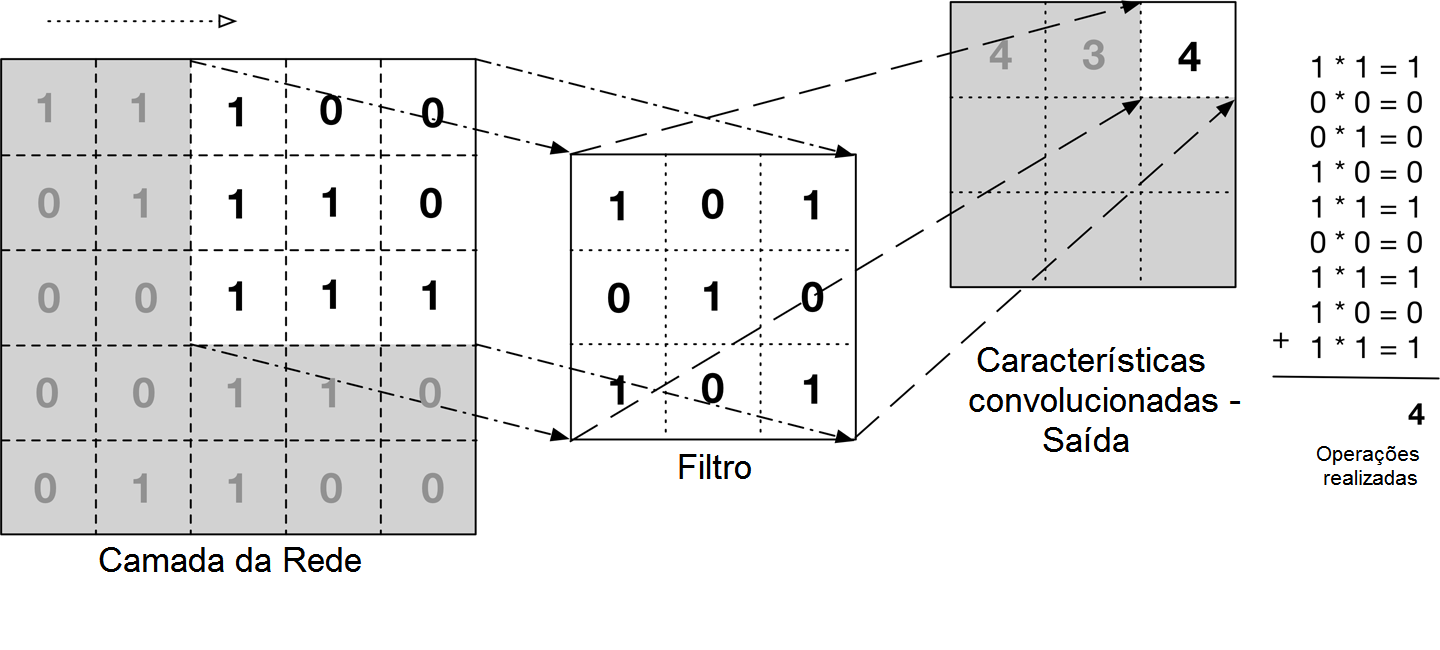
\includegraphics[scale=1.0]{./img/convolucao_matriz_binaria.png}
		\caption{Ilustração do processo de convolução onde se tem a entrada como uma matriz binária, um filtro (que na rede neural faz  papel de pesos sinápticos) e a saída como uma extração das características da matriz de entrada.}
		\label{fig:ConvolutionalOperation}
	\end{figure}
	
	Pode-se pensar, intuitivamente, a convolução como uma operação onde dois sinais são sobrepostos. Com ambos os sinais em mãos, pega-se o primeiro, inverte-se o segundo e faz-se com que este deslise sobre o aquele, e, em cada momento, é calculado o produto interno entre os dois. No fim do processo de "deslisamento", o sinal de saída é gerado. No contexto das redes convolucional, digamos que $X$ seja o sinal de entrada (a entrada da camada convolucional), $W$ seja o filtro desta camada (os pesos sinápticos) e $Y$ a saída. Pode-se então escrever este processo conforme a Equação \ref{eq:ConvolutionalEquation}.
	
	\begin{equation}
	\sigma_{kl} = W_{kl} \cdot X_{i+k,j+l}
	\label{eq:ConvolutionalEquation}
	\end{equation}
	
	Devido às suas características, a CNN é uma boa opção para a classificação de evoluções temporais e se tinha a expectativa de ser uma opção mais robusta quando da aplicação da rede na identificação de evoluções temporais de espaços maiores que o espaço elementar. Mas na solução adotada não se utilizou apenas camadas convolucionais, mas também camadas, inicialmente, densamente conectadas, como ocorre na rede feedforward.
	
	Os resultados utilizando a rede convolucional foram melhores que os obtidos pela rede feedforward. O treinamento foi feito a partir do espaço elementar e a acurácia foi superior a 97\%. Após o treinamento, a rede foi capaz de classificar corretamente todo o espaço elementar através de evoluções temporais apresentadas à rede.
	
	Não é possível apresentar uma classificação a priori do espaço de raio 1,5. Mas em uma avaliação visual preliminar de algumas regras, foi possível perceber que a rede acerta em uma grande quantidade de vezes, falha em outras e oferece resposta inconclusiva para outras tantas. Um problema que foi possível perceber, muito evidente, está relacionado com a classificação de evoluções temporais cujo padrão contém linhas horizontais e verticais que lembram padrões complexos. Para estes casos, apesar da evolução temporal ser claramente periódica, ela é classificada como complexa.
	
	\begin{figure}[H]
		\centering
		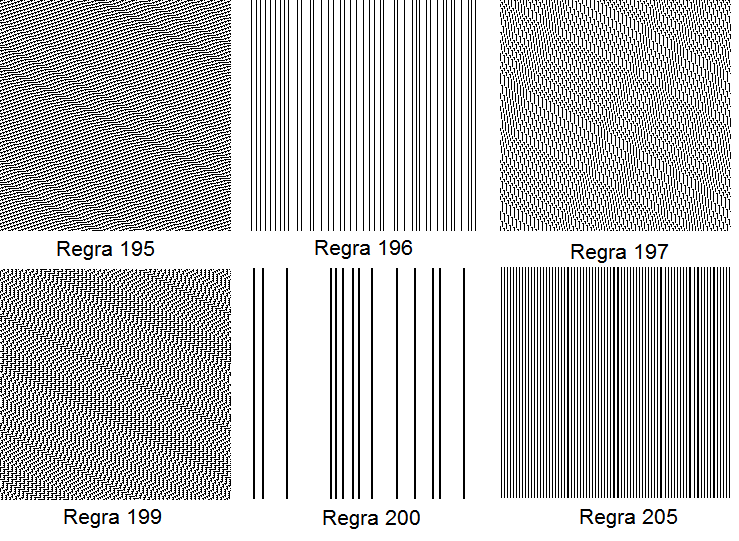
\includegraphics[scale=0.75]{./img/regras_periodicas_diferentes_classificacoes.png}
		\caption{Regras periódicas do espaço de raio 1.5 classificadas de forma distintas pele rede convolucional.}
		\label{fig:PeriodicasDiferentesClassificacoes}
	\end{figure}
	
	A Figura \ref{fig:PeriodicasDiferentesClassificacoes} mostra 6 evoluções temporais do espaço de raio 1.5, cujas regra se encaixariam na classe das regras periódicas, dada uma avaliação visual. No entanto, as regras 195 e 199 foram classificadas como complexas, as regras 196 e 200 foram classificadas como nulas. Mas as regras 197 e 205 foram classificadas, como esperado, periódicas.
	
	A dificuldade na classificação das regras 196 e 200 pode estar relacionado com a estrutura da rede convolucional que extrai características localmente. Como a quantidade de linhas verticais não é muito densa, isso pode levar à conclusão pela rede de que a evolução é nula. O erro para as regras 195 e 199 pode estar relacionado com as linhas diagonais que lembram algumas estruturas complexas que, apesar de irregulares, a localidade das redes convolucionais pode fazer com que se assemelhem.
	
	Trabalha-se com duas possibilidades para lidar com esta dificuldade em classificar algumas evoluções. O número de camadas convolucional pode estar desconsiderando certas características das evoluções temporais, uma vez que a saída de cada camada convolucional diminui não só a dimensão da imagem, como também as característica da mesma. E o processo de dropout também pode estar eliminando conexões com conhecimento sobre as evoluções temporais que é perdida. São necessárioss mais testes com a rede convolucional para se encontrar uma estrutura que melhore a classificação em espaço maiores \cite{NitishSrivastavaEtAl2014}.
	
	
	\chapter{Análise espectral da configuração de vizinhança e determinação automática da classe da regra geradora}
	\label{cap:neighborhoodSpectrumAnalises}
	
	Dada uma evolução temporal é possível calcular um conjunto de métricas denominadas como texturas, no âmbito do processamento de imagem. Tais métricas permitem quantificar percepções da imagem relacionada com a distribuição de cores e intensidade dos pixeis \cite{Stockman:2001}. 
	
	A analise de textura possui duas grandes abordagens; a abordagem estrutural e a abordagem estatística. Na abordagem estrutural analisam-se estruturas que se repetem na imagem, sobre as quais a análise espectral de Fourier pode ser empregada para caracterizar a distribuição das estruturas primitivas. Já a abordagem estatística procura caracterizar as propriedades estocásticas e distribuição espacial dos tons de cinza de uma imagem. As informações da textura da imagem (que está em tons de cinza) são extraídas através da matriz de co-ocorrência, que resulta em uma matriz binária \cite{DongAndLi1990}.
	
	Em \citeonline{DongAndLi1990} foi proposto um tipo de textura que permitiu a determinação de espectros relacionados com os dados desta textura. Usando os espectros, foi possível obter alta acurácia quando aplicada na classificação de imagens relacionadas ao ambiente natural. Tal textura auxiliou a reduzir a quantidade de informações relacionadas à imagem e determinar, com alta acurácia, as classes das imagens.
	
	Os descritores visuais Local Binary Patterns Variance e de Fourrier foram usados em \citeonline{NubiaDaSilva:2016} para classificar ACs binários do espaço elementar, alcançando alta acurácia. E em  \citeonline{Machicao:2018}, além dos descritores Local Binary Patterns e de Fourrier, também foram usados os descritores Gabor e a Matriz de Co-ocorrência em Níveis de Cinza, também alcançando alta acurácia.
	
	Em \citeonline{JassemAndHamid2012} um vetor de características formado pela média da intensidade dos pixeis em cada canal, pelo desvio padrão desta intensidade, por uma medida de assimetria, a entropia e a dimensão da imagem. Esta configuração permitiu classificar imagens com alta acurácia, seja usando a árvore de decisão ou redes neurais. Por tanto é conveniente avaliar se tal vetor se prestaria para a classificação de evoluções temporais.
	
	O primeiro parâmetro é a média da intensidade do pixel em um determinado canal. Uma imagem colorida possui 3 canais, um para cada cor básica. No caso da uma imagem em tons de cinza, há apenas um canal, o que reduz a expressão da média para a forma da Equação \ref{eq:mediaParaUmCanal}, onde j é uma das possíveis intensidades para um pixel.
	
	\begin{equation}
	\mu = \frac{1}{N}\times \sum_{j=0}^{N}P_{j}
	\label{eq:mediaParaUmCanal}
	\end{equation}
	
	Em uma imagem em tons de cinza, entre as 255 intensidades possíveis, algumas podem podem não ocorrer. Mas na evolução temporal, exceto para as regras homogêneas, sempre haverá 0 e 1, fazendo com que $N = 2$ e seja possível reescrever a Equação \ref{eq:mediaParaUmCanal} conforme a Equação \ref{eq:mediaZeroUmConclusao}.
	
	\begin{equation}
	\mu = \frac{1}{2}\times \sum_{j=0}^{2}P_{j}
	\label{eq:mediaZeroUm}
	\end{equation}
	
	\begin{equation}
	\mu = \frac{P_{0}+P_{1}}{2}
	\label{eq:mediaZeroUmConclusao}
	\end{equation}
	
	Como $P_i$ é a proporção entre 0 e 1 na evolução temporal, e exceto pelas homogêneas sempre haverá alguns 1 e alguns 0, se conclui que $P_0 + P_1 = 1$. Logo, para qualquer evolução temporal $\mu = \frac{1}{2}$ e neste caso $\mu$ deixa de ser um parâmetro e passa a ser uma constante, fazendo com que o vetor de característica passe a ter 5 parâmetros ao invés de 6. 
	
	No caso particular deste trabalho as dimensões da imagens são fixas, pois para o treinamento da rede neural a imagem necessita manter suas dimensões. Assim, o vetor de características passa a ter apenas 4 parâmetros, o que desestimulou o uso deste parâmetro como um vetor de característica. Mas a abordagem para a classificação descrita neste capítulo é uma abordagem semelhante.
	
	Apesar de semelhante aos métodos descritos acima, a abordagem descrita neste capítulo é computacionalmente mais simples que os descritores de textura abordados até aqui, mas com acurácia de classificação semelhante.
	
	Uma evolução temporal de um AC binário é uma matriz cujo valores das células são apenas 0 e 1. Tendo em mente a classificação de \citeonline{Wolfram1984} o padrão visual presente na evolução temporal pode variar muito devido às quatro classes nas quais as regras podem estar presentes e também pela variabilidade devido à escolha da condição inicial. 
	
	Porém, encarando a evolução temporal como uma imagem binária, conforme feito nos capítulos anteriores, e analisando esta imagem localmente em torno de um pixel; uma célula da evolução temporal, percebem-se padrões repetitivos na configuração da vizinhança desta célula.
	
	Escolhendo um raio $r$ ao redor de uma célula em uma configuração de vizinhança de Moore, haverá $(2r + 1)^2$ células nesta vizinhança, que se traduz em $2^{(2r + 1)^2}$ possibilidades de configurações distintas para uma imagem binária \cite{http://mathworld.wolfram.com-01}.
	
	Mantendo uma correspondência com o espaço elementar e fazendo $r = 1$, haverá 9 células na vizinhança e $2^9 = 512$ possíveis configurações de vizinhanças diferentes. Ou seja, por mais caótico que seja o padrão da evolução temporal, haverá apenas 512 configurações possíveis na vizinhança de uma célula.
	
	Tal fato abre a possibilidade de uma classificação automática ao se extrair um vetor de característica de uma evolução temporal, contando o número de ocorrência de cada configuração de vizinhança e normalizando esta contagem. Assim se obtém um Espectro da Configuração de Vizinhança de uma evolução temporal.
	
	A proposta de classificação apresentada neste capítulo baseia-se na hipótese de que dado um vetor $\vec{c}=\{c_0,c_1,...,c_{511}\}$ que representa um Espectro da Configuração de Vizinhança de uma evolução temporal binária qualquer, pode ser classificado se utilizando um conjunto de vetores $\vec{c_n}=\{c_{n,0},c_{n,1},...,c_{n,511}\}$, Espectros de Configuração de Vizinhança de um conjunto de evoluções temporais geradas por cada regra $n$ do espaço elementar. A classe $\vec{c}$ poderia ser identificada se buscando $min(dist(\vec{c},\vec{c_n}))$.
	
	Além da identificação da evolução temporal gerada por uma regra do espaço elementar, tem-se como uma segunda hipótese, a possibilidade de se aplicar a mesma técnica em evoluções temporais geradas por regras de espaços maiores, devido ao fato de que nenhuma característica intrínseca do espaço elementar foi levado em conta para gerar os vetores $\vec{c_n}$ ou o vetor $\vec{c}$.
	
	Para se testar as hipóteses, foi gerado um conjunto de vetores, um para cada regra do espaço elementar ($B=\{c_0,c_1,c_2...,c_{255}\}$). Para cada regra foram geradas 100 condições iniciais aleatórias, para as quais o espectro foi calculado.
	
	Para uma avaliação inicial foi gerada apenas uma evolução temporal para cada regra do espaço elementar e se comparou a classificação feita automaticamente com a classificação conhecida do espaço elementar. 
	
	A distância utilizada na busca pode levantar questões sobre a capacidade de discriminação do processo. Uma questão óbvia sobre o comportamento espectral das regras dinamicamente equivalentes se impõe, pois poderia se esperar que os espectros sejam iguais, devido à equivalência dinâmica.
	
	Apesar de ainda não conclusivas, uma avaliação preliminar dos espectros obtidos a partir do espaço elementar sugere que tal problema de discriminação das regras equivalentes não existe, como sugerem as Figuras \ref{fig:EspectroRegra41} e \ref{fig:EspectroRegra97}
	
	\begin{figure}[H]
		\centering
		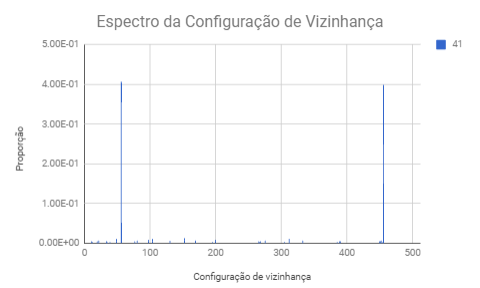
\includegraphics[scale=0.75]{./img/espectro_regra_41.png}
		\caption{Espectro da Configuração de Vizinhança da regra 41 do espaço elementar}
		\label{fig:EspectroRegra41}
	\end{figure}
	
	\begin{figure}[H]
		\centering
		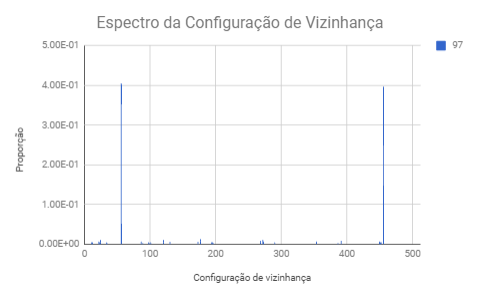
\includegraphics[scale=0.75]{./img/espectro_regra_97.png}
		\caption{Espectro da Configuração de Vizinhança da regra 97 do espaço elementar}
		\label{fig:EspectroRegra97}
	\end{figure}
	
	Ambas as regras são dinamicamente equivalentes, os espectros de ambas são semelhantes, mas os detalhes na configuração do espectro em torno dos pontos 100, 200, 300 e 400, deixa clara as diferenças. E ao se calcular a distância entre os dois vetores se percebe que apesar de serem dinamicamente equivalentes, a distância entre os dois vetores de 56.003 permite diferenciá-los perfeitamente.
	
	Após gerar a classificação do espaço elementar foi possível observar que para as regras 104 e 233 o acerto ficou em 70\%, para as regras 36 e 41, o acerto foi de 80\% e para as regras 72, 107, 164, 219 e 237 o acerto ficou em 90\%. Todas as demais regras o método acerta 100\% das vezes.
	
	No contexto geral, esta estratégia de classificação se mostrou promissora não só devido à acurácia alcançada, mas também por ser relativamente mais simples, comparando-se à utilização de redes neurais como exposto nos capítulos anteriores.
	
	Também foi feita uma comparação entre os dois métodos desenvolvidos, comparando-se a classificação a que cada um chegou. Até onde esta correspondência pode ser verificada, se observou, com pouco mais de 60\% de concordância entre os dois métodos.
	
	
	\chapter{Análise dos resultados}
	\label{cap:resultados}
	
	Classificar ACs binários se mostrou um tarefa mais complexa que a classificação de imagens, apesar de a evolução temporal poder ser tratada como uma imagem binária e esta ser muito mais simples que uma outra colorida. O desafio está no fato de que ACs gerados por uma mesma classe podem ter seu padrão visual muito variado, indo além do que se encara como ruído em uma imagem normal, chegando mesmo a classificar uma evolução temporal com uma classe distinta da regra geradora. Isso ocorre, por exemplo, em regras caóticas, que, para determinados tamanhos ou configurações iniciais, se comportam como regras nulas.
	
	Neste trabalho os maiores esforços para a classificação foram feitos através de redes neurais artificiais de dois tipos; as redes feedforward e convolucionais. Também foi feito um esforço para compreender a estrutura das evoluções temporais típicas das regras do espaço elementar, gerando uma base de dados dos espectros destas evoluções. Esta base mostrou-se útil na classificação por proximidade espacial, calculando-se a distância euclidiana entre um espectro gerado a partir de uma evolução temporal qualquer e os da base de espectros. A Seção \ref{ResultadosObtidoUsoRedesNeurais} descreveu os resultados obtidos utilizando as redes neurais e a Seção \ref{ResultadosObtidoUsoBaseEspectros} descreveu os resultados com a base de dados dos espectros.
	
	
	\section{Resultados Obtidos com o Uso de Redes Neurais}
	\label{ResultadosObtidoUsoRedesNeurais}
	
	No Capítulo \ref{cap:classACUsingNetwork} discutiu-se a aplicação de redes neurais artificiais na classificação de ACs binários, onde foi mostrado algumas estruturas de rede e dados utilizados na classificação. Entre as rede utilizadas a convolucional obteve melhores resultados não só no treinamento, mas após a rede treinada, também em sua utilização.
	
	Após o treinamento e determinação da acurácia o primeiro uso da rede convolucional foi classificar o espaço elementar. Uma vez que todas as redes foram treinadas com evoluções temporais deste espaço, esperava-se acerto na classificação de todas as regras, mas isto só foi observado na rede convolucional.  
	
	A Tabela \ref{table:regrasClassificadasCNN} apresenta um corte da classificação obtida pela rede. Nela as duas primeiras colunas são a regra e sua classe, a coluna Classe Predita é a classificação predita pela rede e as colunas $c_i$ são as probabilidades de a regra ser da classe 1, 2, 3 ou 4. Para predizer a classe, escolhia-se a mesma numeração da coluna $c_i$ com maior probabilidade.
	
	\begin{table}[H]
		\centering
		\caption{Regras do espaço elementar classificadas corretamente com rede neural artificial convolucional.
		}
		\label{table:regrasClassificadasCNN}
		\vskip 0.3cm
		\begin{tabular}{ c c c l l l l }
			\hline
			Regra & Classe & Classe Predita & c1 & c2 & c3 & c4 \\ \hline
			160 & 1 & 1 & 0.99375 & 0.00618 & 0.00004 & 0.00002 \\ \hline
			161 & 3 & 3 & 0.19899 & 0.00101 & 0.79979 & 0.00021 \\ \hline
			162 & 2 & 2 & 0.19875 & 0.80096 & 0.00001 & 0.00029 \\ \hline
			163 & 2 & 2 & 0.19899 & 0.80077 & 0.00000 & 0.00024 \\ \hline
			164 & 2 & 2 & 0.19893 & 0.80102 & 0.00003 & 0.00002 \\ \hline
			165 & 3 & 3 & 0.19899 & 0.00102 & 0.79998 & 0.00002 \\ \hline
			166 & 2 & 2 & 0.19875 & 0.79789 & 0.00001 & 0.00335 \\ \hline
			167 & 2 & 2 & 0.19899 & 0.70253 & 0.02038 & 0.07810 \\ \hline
			168 & 1 & 1 & 0.99375 & 0.00618 & 0.00004 & 0.00002 \\ \hline
			169 & 4 & 4 & 0.19899 & 0.00120 & 0.00005 & 0.79976 \\ \hline
		\end{tabular}
	\end{table}
	
	Naturalmente, pode ocorrer de uma regra ser classificada com baixa probabilidade como $0.4$, porém a menor observada foi $0.67964$ ao classificar a regra 237.
	
	Ao aplicar o mesmo processo ao espaço de raio r=1.5, apesar de não haver uma classificação prévia que se possa utilizar para comparação, observou-se algumas inconsistências. A regra 14 foi classificada como caótica, quando sua aparência e de uma regra periódica, como pode-se ver na Figura \ref{fig:regra14r1.5}. A regra 21423 foi classificada como periódica, mas sua aparência lembra uma regra complexa, como pode-se ver na Figura \ref{fig:regra21423r1.5}. Já a regra 21391 aparentemente foi classificada corretamente como complexa, Figura \ref{fig:regra21391r1.5}. No entanto vale salientar que para a regra 21391 sua probabilidade foi de apenas 0.56975, sendo que a de ser periódica foi de 0.43006.
	
	\begin{figure}[H]
		\centering
		
\includegraphics[scale=1.0]{./img/ca_sample_14.png}
		\caption{Evolução temporal da regra 14 do espaço de raio r=1.5}
		\label{fig:regra14r1.5}
	\end{figure}
	
	\begin{figure}[H]
		\centering
		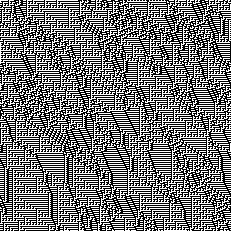
\includegraphics[scale=1.0]{./img/ca_sample_21391.png}
		\caption{Evolução temporal da regra 21391 do espaço de raio r=1.5}
		\label{fig:regra21391r1.5}
	\end{figure}
	
	\begin{figure}[H]
		\centering
		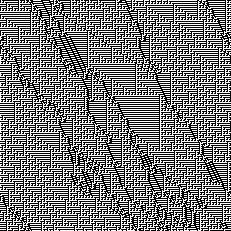
\includegraphics[scale=1.0]{./img/ca_sample_21423.png}
		\caption{Evolução temporal da regra 21423 do espaço de raio r=1.5}
		\label{fig:regra21423r1.5}
	\end{figure}
	
	Pela classificação obtida observou-se uma dificuldade da rede em classificar as regras complexas. A suposição é de que ela identifica a estrutura complexa da evolução temporal nestes casos como as mesmas observadas para as regras periódicas. Ou seja, a rede encara como semelhantes as linhas diagonais como as da regra 14, como as estruturas complexas diagonais das regras 21423 e  21391. Curiosamente, o mesmo não ocorreu quando o espaço de raio r=1.0 foi classificado. Isso leva à questão de, que no caso do espaço de raio r=1.5, pode-se estar observando características dinâmicas não observadas no espaço elementar.
	
	Na próxima seção será abordado outro método de classificação baseado na configuração da vizinhança de uma célula e na obtenção da frequência com que cada configuração possível ocorre na evolução temporal; bons resultados foram obtidos na classificação tanto do espaço elementar, quanto do de raio r=1.5.
	
	\section{Resultados Obtidos com o Uso do Conjunto de Espectros}
	\label{ResultadosObtidoUsoBaseEspectros}
	
	O Espectro da Configuração de Vizinhança oferece um meio para se conhecer melhor o comportamento das evoluções temporais típicas geradas pelas regras do espaço elementar. Em um primeiro momento se poderia usar o espectro como um vetor de características a ser utilizado como entrada em uma rede neural, mas tal estrutura se mostrou muito útil na classificação usando a distância euclidiana entre um espectro qualquer e o conjunto de espectros gerados para o espaço elementar.
	
	É importante salientar que, a não ser que se assuma a inclusão de novos espectros como um tipo particular, a classificação neste caso não se baseou em aprendizado de máquina. O importante aqui é o acumulo de espectros em um conjunto que serve como base de comparação com outros fora do conjunto. No entanto há uma proximidade com o aprendizado de máquina devido à flexibilidade do que é possível alcançar com esta técnica.
	
	Assim como uma rede neural que erre a classificação de uma evolução temporal, também pode-se incluir no conjunto de espectros, outros que não estão presentes, aumentando a capacidade de reconhecimento ao usar o novo conjunto. Isso quer dizer que ao ser aplicado em espaços maiores, ao se encontrar uma classificação que não esteja de acordo com o esperado ou classificado por outros métodos, pode-se gerar o espectro desta regra, aumentando a acurácia. 
	
	Dito isto, faz-se necessário abordar a acurácia desta técnica. Como descrito antes, aqui o processo automático toma por base a classificação de \citeonline{Wolfram1984} e procura levá-la para espaços maiores. Após a geração do conjunto de espectros para cada regra do espaço elementar, procedeu-se com a classificação do mesmo utilizando o conjunto. Considerou-se um limiar acima da proporção de acerto de 50\% para considerar a classificação como correta e a acurácia foi de 100\%. Ou seja, todas as regras obtiveram proporção de acerto acima do limiar. Apenas 28 regras não obtiveram 100\% de acerto na classificação, dentre elas a regra 104, da classe 2, obteve 85.4\% de classificações corretas e a regra 151, da classe 3, foi classificada corretamente 99.8\% das vezes. A Tabela \ref{table:regrasClassificadasSpectroErro}, mostra a lista completa deste conjunto de regras. No total 18 são da classe 2, 2 da classe 3 e 8 da classe 4. Evidencia-se uma maior propensão a falhas relacionadas a regra 2 e nenhuma falha entre as homogêneas.

    \begin{table}[htbp]
		\centering
		\caption{Regras do espaço elementar classificadas corretamente com o espectro de configuração de vizinhança, mas que não houve total concordância com a classe real.
		}
		\label{table:regrasClassificadasSpectroErro}
        \makebox[\textwidth][c]{
        \begin{tabular}{ccc|ccc}
            \toprule
    		\hline
    		\hline
    		Regra & Classe & Proporção & Regra & Classe & Proporção\\ \hline
    		104 & 2 & 0.854 & 82 & 2 & 0.986 \\ \hline
    		233 & 2 & 0.874 & 183 & 3 & 0.986 \\ \hline
    		36 & 2 & 0.884 & 164 & 2 & 0.988 \\ \hline
    		121 & 4 & 0.898 & 225 & 4 & 0.988 \\ \hline
    		107 & 4 & 0.902 & 237 & 2 & 0.988 \\ \hline
    		219 & 2 & 0.916 & 26 & 2 & 0.990 \\ \hline
    		41 & 4 & 0.924 & 111 & 2 & 0.992 \\ \hline
    		97 & 4 & 0.934 & 125 & 2 & 0.992 \\ \hline
    		106 & 4 & 0.956 & 181 & 2 & 0.994 \\ \hline
    		120 & 4 & 0.974 & 9 & 2 & 0.996 \\ \hline
    		218 & 2 & 0.976 & 223 & 2 & 0.996 \\ \hline
    		72 & 2 & 0.978 & 4 & 2 & 0.998 \\ \hline
    		167 & 2 & 0.984 & 103 & 2 & 0.998 \\ \hline
    		169 & 4 & 0.984 & 151 & 3 & 0.998 \\ \hline
    		\hline
            \bottomrule
        \end{tabular}%
        }
    \end{table}%

	Ao aplicar a mesma técnica de classificação no espaço com raio 1.5 não há como definir a acurácia, pois não há uma classificação conhecida do espaço de raio 1.5 para comparação. Mas uma inspeção nas evoluções temporais obtidas e comparando com as classificações observa-se que as regras 14 e 21423 foram classificadas como periódicas e a 21391 complexa. Mas, observando as evoluções temporais das Figuras \ref{fig:regra14r1.5}, \ref{fig:regra21391r1.5} e \ref{fig:regra21423r1.5}, percebe-se que as regras 21391 e 21423 tem evolução temporal aparentemente complexa, enquanto a 14 é periódica. A verificação foi visual e mostrou que ao aplicar a estratégia em um espaço maior houve erro, apesar de não se poder aferir a acurácia na classificação do espaço, ocorrendo o mesmo ao usar redes neurais, como se viu na seção anterior.
	
	A primeira impressão sobre o uso do espectro de vizinhança é uma acurácia semelhante à rede convolucional e talvez isto mostre que as erros semelhantes para as regras aparentemente complexas do espaço de raio r=1.5 indique comportamento dinâmico não presentes no espaço elementar.
	
	A próxima seção compara os dois métodos para medir a concordância entre ambos, oferecendo uma primeira avaliação, se aplicar ambos os processos de classificação em espaços maiores oferece uma acurácia boa o suficiente para que sejam adotados.
	
	\section{Comparação entre as Classificações via Rede Neural e Conjunto de Espectros}
	\label{ComparacaoClassificacoesRedeNeuralConjuntoEspectros}
	
	Para avaliar a concordância dos métodos, foram geradas 500 evoluções temporais para cada regra do espaço de r = 1.5, onde cada uma delas foram classificadas por ambas as estratégias, a partir do que calculou-se a proporção de vezes que ambos os métodos concordaram. E foi observado que os dois métodos guardaram certa concordância na classificação das evoluções temporais do espaço de raio r=1.5 com 47102 regras recebendo a mesma classificação de ambos e 18434 com classificações distintas. Estes números resultam em 71.9\% de concordância entre ambos. No entanto, como foi mostrado nas duas seções anteriores, ambos podem estar errados na classificação obtida e na parcela em que discordam, já que um dos dois métodos pode estar incorreto.
	
	Não há como avaliar qual método possui melhor acurácia para o espaço de raio r=1.5, pois não há uma classificação prévia para comparação. Porém, é possível corrigir os resultados com o intuito de se verificar onde cada método é mais frágil, realimentá-los, e obter uma melhor acurácia. E isso vale para qualquer espaço maior que o elementar.

	Não é possível predizer uma acurácia esperada para cada espaço particular. Levando em consideração que espaços maiores podem apresentar comportamentos dinâmicos que não estão presentes no espaço elementar, usado com referência, ambos os métodos são capazes de classificar com boa taxa de acurácia os comportamentos observados no espaço elementar e aqueles não encontrados nele, que não foram bem classificados, podem realimentar a ambos para aumentar suas acurácias.
	
	No entanto, diante dos resultados obtidos e da simplicidade da análise do espectro de vizinhança, se comparado à rede neural, a análise do espectro de vizinhança, por seu custo computacional menor apresenta-se como uma melhor opção na classificação de Autômatos Celulares binários. 
	
	
	\chapter{Conclusão e cronograma}
	\label{cap:conclusaoCronograma}
	
	Neste trabalho abordaram-se duas formas de se classificar autômatos celulares automaticamente usando as regras do espaço elementar classificado segundo a classificação de \citeonline{Wolfram1984}. A rede neural associou a cada evolução temporal apresentada uma das 4 classes, enquanto a análise do espectro de vizinhança associa primeiro a uma regra do espaço elementar para então se chegar a conclusão da classe.
	
	Tanto o uso da rede convolucional quanto o espectro de vizinhança mostraram grande acurácia, mas o uso do espectro para se fazer a classificação mostrou-se menos custoso. No entanto a comparação entre os dois métodos no espaço de raio 1.5 é inconclusivo, uma vez que não há base para comparação. Obter a classificação deste espaço auxiliaria na determinação da acurácia para o espaço de raio 1.5.
	
	Nos próximos meses as tarefas a serem concluídas são a escrita dos artigos para publicação, publicação e obtenção do aceite. Paralelo a isso, classificar as regras do espaço de raio 1.5 que permitirá comparação com os métodos obtidos aqui. Na sequência, será feita a escrita da tese, o depósito e sua defesa. O cronograma a seguir, detalha as datas e tempo para cada atividade.
	
	\begin{figure}[H]
		\centering
		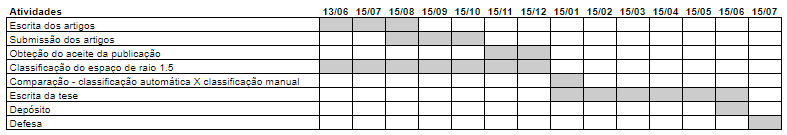
\includegraphics[scale=0.75]{./img/cronograma.png}
		\label{fig:cronograma}
	\end{figure}
	
	\def\refname{Referências Bibliográficas}
	\bibliography{biblproj}
	\addcontentsline{toc}{section}{REFERÊNCIAS BIBLIOGRÁFICAS}
	\bibliographystyle{abntex2-alf}
	
\end{document}
